\ifdefined\ishandout
  \documentclass[handout,landscape]{beamer} 
\else
  \documentclass[landscape]{beamer}
\fi

%\hypersetup{pdfpagemode=FullScreen} %Enabling this option will cause the slides to go full-screen on opening

\mode<handout>
{
  \usepackage{pgf}
  \usepackage{pgfpages}

\pgfpagesdeclarelayout{6 on 1 boxed}
{
  \edef\pgfpageoptionheight{\the\paperheight} 
  \edef\pgfpageoptionwidth{\the\paperwidth}
  \edef\pgfpageoptionborder{0pt}
}
{
  \pgfpagesphysicalpageoptions
  {%
    logical pages=6,%
    physical height=\pgfpageoptionheight,%
    physical width=\pgfpageoptionwidth%
  }
  \pgfpageslogicalpageoptions{1}
  {%
    border code=\pgfsetlinewidth{2pt}\pgfstroke,%
    border shrink=\pgfpageoptionborder,%
    resized width=.5\pgfphysicalwidth,%
    resized height=.5\pgfphysicalheight,%
    center=\pgfpoint{.25\pgfphysicalwidth}{.833\pgfphysicalheight}%
  }%
  \pgfpageslogicalpageoptions{2}
  {%
    border code=\pgfsetlinewidth{2pt}\pgfstroke,%
    border shrink=\pgfpageoptionborder,%
    resized width=.5\pgfphysicalwidth,%
    resized height=.5\pgfphysicalheight,%
    center=\pgfpoint{.75\pgfphysicalwidth}{.833\pgfphysicalheight}%
  }%
  \pgfpageslogicalpageoptions{3}
  {%
    border code=\pgfsetlinewidth{2pt}\pgfstroke,%
    border shrink=\pgfpageoptionborder,%
    resized width=.5\pgfphysicalwidth,%
    resized height=.5\pgfphysicalheight,%
    center=\pgfpoint{.25\pgfphysicalwidth}{.5\pgfphysicalheight}%
  }%
  \pgfpageslogicalpageoptions{4}
  {%
    border code=\pgfsetlinewidth{2pt}\pgfstroke,%
    border shrink=\pgfpageoptionborder,%
    resized width=.5\pgfphysicalwidth,%
    resized height=.5\pgfphysicalheight,%
    center=\pgfpoint{.75\pgfphysicalwidth}{.5\pgfphysicalheight}%
  }%
  \pgfpageslogicalpageoptions{5}
  {%
    border code=\pgfsetlinewidth{2pt}\pgfstroke,%
    border shrink=\pgfpageoptionborder,%
    resized width=.5\pgfphysicalwidth,%
    resized height=.5\pgfphysicalheight,%
    center=\pgfpoint{.25\pgfphysicalwidth}{.167\pgfphysicalheight}%
  }%
  \pgfpageslogicalpageoptions{6}
  {%
    border code=\pgfsetlinewidth{2pt}\pgfstroke,%
    border shrink=\pgfpageoptionborder,%
    resized width=.5\pgfphysicalwidth,%
    resized height=.5\pgfphysicalheight,%
    center=\pgfpoint{.75\pgfphysicalwidth}{.167\pgfphysicalheight}%
  }%
}


  \pgfpagesuselayout{6 on 1 boxed}[letterpaper, border shrink=5mm]
  \nofiles
}

\usepackage{listings}
\usepackage{multimedia}
\usepackage[normalem]{ulem}
\usepackage{ifthen}

\usetheme{Warsaw} 
\usecolortheme{seahorse}
\useoutertheme{infolines} 

\setbeamertemplate{blocks}[rounded][shadow=true] 

\author{Joe Fields}
\title{Introduction to Proof} 

\date{Lecture 24 (GIAM \S 4.5) \newline Russell's paradox}
\institute[SCSU]{ {\tt fieldsj1@southernct.edu} }

\newcommand{\versionNum}{$3.2$\ }

\newboolean{InTextBook}
\setboolean{InTextBook}{false}
\newboolean{InWorkBook}
\setboolean{InWorkBook}{false}
\newboolean{InHints}
\setboolean{InHints}{false}

%When this boolean is true (beginning in Section 5.1) we will use the convention
% that $0 \in \Naturals$.  If it is false we will continue to count $1$ as the smallest
%natural number (thus making Giuseppe Peano spin in his grave...)
 
\newboolean{ZeroInNaturals}

%This boolean is used to distinguish the version where we use $\sim$ rather than $\lnot$

\newboolean{LNotIsSim}

%The values of the last two booleans are set in ``switches.tex''

\setboolean{ZeroInNaturals}{true}
\setboolean{LNotIsSim}{false}


\let\savedlnot\lnot
\ifthenelse{\boolean{LNotIsSim}}{\renewcommand{\lnot}{\sim} }{}

%This command puts different amounts of space depending on whether we are
% in the text, the workbook or the hints & solutions manual. 
\newcommand{\twsvspace}[3]{%
 \ifthenelse{\boolean{InTextBook} }{\vspace{#1}}{%
  \ifthenelse{\boolean{InWorkBook} }{\vspace{#2}}{%
   \ifthenelse{\boolean{InHints} }{\vspace{#3}}{} %
   }%
  }%
 }


\newcommand{\wbvfill}{\ifthenelse{\boolean{InWorkBook}}{\vfill}{}}
\newcommand{\wbitemsep}{\ifthenelse{\boolean{InWorkBook} }{\rule[-24pt]{0pt}{60pt}}{}}
\newcommand{\textbookpagebreak}{\ifthenelse{\boolean{InTextBook}}{\newpage}{}}
\newcommand{\workbookpagebreak}{\ifthenelse{\boolean{InWorkBook}}{\newpage}{}}
\newcommand{\hintspagebreak}{\ifthenelse{\boolean{InHints}}{\newpage}{}}

\newcommand{\hint}[1]{\ifthenelse{\boolean{InHints}}{ {\par \hspace{12pt} \color[rgb]{0,0,1} #1 } }{}}
\newcommand{\inlinehint}[1]{\ifthenelse{\boolean{InHints}}{ { \color[rgb]{0,0,1} #1 } }{}}

\newlength{\cwidth}
\newcommand{\cents}{\settowidth{\cwidth}{c}%
\divide\cwidth by2
\advance\cwidth by-.1pt
c\kern-\cwidth
\vrule width .1pt depth.2ex height1.2ex
\kern\cwidth}

\newcommand{\sageprompt}{ {\tt sage$>$} }
\newcommand{\tab}{\rule{20pt}{0pt}}
\newcommand{\blnk}{\rule{1.5pt}{0pt}\rule{.4pt}{1.2pt}\rule{9pt}{.4pt}\rule{.4pt}{1.2pt}\rule{1.5pt}{0pt}}
\newcommand{\suchthat}{\; \rule[-3pt]{.5pt}{13pt} \;}
\newcommand{\divides}{\!\mid\!}
\newcommand{\tdiv}{\; \mbox{div} \;}
\newcommand{\restrict}[2]{#1 \,\rule[-4pt]{.25pt}{14pt}_{\,#2}}
\newcommand{\lcm}[2]{\mbox{lcm} (#1, #2)}
\renewcommand{\gcd}[2]{\mbox{gcd} (#1, #2)}
\newcommand{\Naturals}{{\mathbb N}}
\newcommand{\Integers}{{\mathbb Z}}
\newcommand{\Znoneg}{{\mathbb Z}^{\mbox{\tiny noneg}}}
\ifthenelse{\boolean{ZeroInNaturals}}{%
  \newcommand{\Zplus}{{\mathbb Z}^+} }{%
  \newcommand{\Zplus}{{\mathbb N}} }
\newcommand{\Enoneg}{{\mathbb E}^{\mbox{\tiny noneg}}}
\newcommand{\Qnoneg}{{\mathbb Q}^{\mbox{\tiny noneg}}}
\newcommand{\Rnoneg}{{\mathbb R}^{\mbox{\tiny noneg}}}
\newcommand{\Rationals}{{\mathbb Q}}
\newcommand{\Reals}{{\mathbb R}}
\newcommand{\Complexes}{{\mathbb C}}
%\newcommand{\F2}{{\mathbb F}_{2}}
\newcommand{\relQ}{\mbox{\textsf Q}}
\newcommand{\relR}{\mbox{\textsf R}}
\newcommand{\nrelR}{\mbox{\raisebox{1pt}{$\not$}\rule{1pt}{0pt}{\textsf R}}}
\newcommand{\relS}{\mbox{\textsf S}}
\newcommand{\relA}{\mbox{\textsf A}}
\newcommand{\Dom}[1]{\mbox{Dom}(#1)}
\newcommand{\Cod}[1]{\mbox{Cod}(#1)}
\newcommand{\Rng}[1]{\mbox{Rng}(#1)}

\DeclareMathOperator\caret{\raisebox{1ex}{$\scriptstyle\wedge$}}

\newtheorem*{defi}{Definition}
\newtheorem*{exer}{Exercise}
\newtheorem{thm}{Theorem}[section]
\newtheorem*{thm*}{Theorem}
\newtheorem{lem}[thm]{Lemma}
\newtheorem*{lem*}{Lemma}
\newtheorem{cor}{Corollary}
\newtheorem{conj}{Conjecture}

\renewenvironment{proof}%
{\begin{quote} \emph{Proof:} }%
{\rule{0pt}{0pt} \newline \rule{0pt}{15pt} \hfill Q.E.D. \end{quote}}


\newcommand{\vs}{\rule{0pt}{12pt}}
\newcommand{\notimplies}{\;\not\!\!\!\implies}

\AtBeginSection[]
{
 \begin{frame}{Table of Contents} 
  \tableofcontents[currentsection]
 \end{frame}
}

%%%% SAVE %%%%
%{ %magic to get a full screen image...
%\setbeamertemplate{navigation symbols}{}  % hide navigation buttons 
%\setbeamertemplate{background canvas}{\centerline{\includegraphics 
%	[height=\paperheight]{Cantor_4.jpeg}}}
%\begin{frame}[plain]
%\rule{0pt}{0pt}
%\end{frame} 
%} %end of magic


\begin{document}

\begin{frame}[plain]
  \titlepage
\end{frame}

\section{Bertrand Russell}

{ %magic to get a full screen image...
\setbeamertemplate{navigation symbols}{}  % hide navigation buttons 
\setbeamertemplate{background canvas}{\centerline{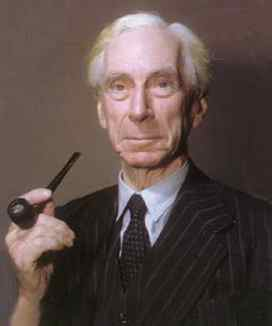
\includegraphics 
	[height=\paperheight]{Russell_4.jpeg}}}
\begin{frame}[plain]
\rule{0pt}{0pt}
\end{frame} 
} %end of magic


\begin{frame}{Bertrand Russell}
\begin{itemize}
\item Bertrand Russell, 1872--1970\pause
\item Discovered the paradox in 1901. \pause
\item pacifist / anti-war activist / anti-nuclear activist \pause
\item Dismissed from Trinity College in 1916 \pause
\item {\em Principia Mathematica} \pause (the other one) \pause
\item The defence of logicism \pause
\item Dismissed from City College, New York as ``morally unfit to teach at the College''\pause
\item the Nobel Prize for Literature in 1950 \pause
\item the Russell-Einstein Manifesto in 1955 \pause
\item Twice imprisoned for his protest efforts (the 2nd time at age 88!) 
\end{itemize}
\end{frame}

\section{the set of all sets}

\begin{frame}{can a set contain itself?}
\begin{itemize}
\item<1-> Inside the set of all sets there is a pathological condition that we would like to avoid. 
\item<2-> If a set $A$ contains itself (as an element) we get a strange infinite regress. 
\item<3-> Example --  If $A \; = \; \{1, 2, A \}$, we can expand that as follows: 
\begin{align*}
\uncover<4->{A \; & = \; \{1, 2, A \} \\ }
\uncover<5->{A \; & = \; \{1, 2, \{1, 2, A \} \} \\ }
\uncover<6->{A \; & = \; \{1, 2, \{1, 2, \{1, 2, A \} \} \} \\ }
\uncover<7->{A \; & = \; \{1, 2, \{1, 2, \{1, 2, \{1, 2, A \} \} \} \} \\ }
\uncover<8->{    & \mbox{et cetera} }
\end{align*}
\item<9-> So mathematicians chose to work in the set of all sets that don't contain themselves.

\end{itemize}
\end{frame}

\begin{frame}{well-defined?}
\begin{itemize}
\item The ``set of all sets'' would appear on its surface to be well defined. \pause
\item The membership criterion would be $P(x) \; = $ ``$x$ is a set'' \pause
\item Can't we always tell whether a thing is a set or not? \pause
\item And amongst those things that are sets, surely we can tell whether they contain themselves (or not).  
\end{itemize}
\end{frame}

\section{the barber paradox}

\begin{frame}{who shaves the barber?}
\begin{itemize}
\item The barber paradox exhibits the same issue that's at the heart of Russell's paradox but is considered easier. \pause
\item The setup sounds sexist and weird to modern ears.  Just remember this is from over 100 years ago.  \pause
\item Also, the razors you're most likely to be familiar with bear little resemblance to the straight razors used in that era. They were dangerous! \pause
\item {\bf In a small town, the Barber shaves all those men (and only those men) who don't shave themselves.} \pause
\item Who shaves the barber?
\end{itemize}
\end{frame}

\begin{frame}{what's the paradox?}
\begin{itemize}
\item If the Barber doesn't shave himself, then he's one of the people that he is supposed to shave. \pause
\item If he {\em does} shave himself then he's one of the people he's not supposed to be shaving. \pause
\item Let $P(x)$ be ``$x$ shaves himself.''
\item For the Barber ($b$) we have:
\[ P(b) \, \implies \, \lnot P(b) \; \land \; \lnot P(b) \, \implies \, P(b). \] \pause
\item In other words (or rather, symbols):
\[ P(b) \, \iff \, \lnot P(b). \]
\end{itemize}
\end{frame}

\begin{frame}{again?}
\begin{itemize}
\item<1-> If a statement implies its own negation, it could just be that the statement is false. 
\item<2-> When a statement implies its negation {\bf and} the negation implies the original\textellipsis 
\item<3-> We get stuck in an infinite loop. 
\item<4-> We can also use logical equivalences to see that what we're dealing with is a contradiction. 
\begin{align*}
\uncover<5->{ & P \, \implies \, \lnot P  \; \land \; \lnot P \, \implies \, P & & \mbox{Given} \\ }
\uncover<6->{  & (\lnot P \, \lor \, \lnot P)  \; \land \; (P \, \lor \, P)     & & \mbox{Disjunctive form of conditional} \\ }
\uncover<7->{  & \lnot P \; \land \; P                                          & & \mbox{Idempotence} \\ }
\uncover<8->{  & c                                                            & & \mbox{Complementarity} \\ }
\end{align*}
\end{itemize}
\end{frame}


\section{Russell's paradox}

\begin{frame}{the setup}
\begin{itemize}
\item Russell's paradox is concerned with the set of all sets that do not contain themselves as elements. \pause
\item Let $S$ be the set of all sets that don't contain themselves as elements, \pause
\[ S \; = \; \{ A \, \suchthat \, A \; \mbox{is a set} \; \land A \notin A \}. \] \pause
\item In the barber's paradox, there is an ``inconvenient question'' -- Who shaves the barber? \pause
\item Here, the inconvenient question is -- Is $S \in S$? 
\end{itemize}
\end{frame}

\begin{frame}{the punchline}
\begin{itemize}
\item There are just two possibilities: either $S \in S$ or $S \notin S$. \pause
\item But, if $S \in S$, then $S$ must satisfy the membership criterion for $S$, which is that $S \notin S$! \pause
\item On the other hand, if $S \notin S$ then $S$ does indeed satisfy the membership criterion for $S$, so $S \in S$! \pause
\item So we have $P \iff \lnot P$ where $P$ is the statement $S \in S$.

\end{itemize}
\end{frame}

\section{Resolution}

\begin{frame}{what now?}
\begin{itemize}
\item So, set theory is pretty much the foundation of all mathematics, and set theory has a nasty contradiction hidden in its foundations. \pause
\item The principle of explosion. \pause
\item Russell's solution was to develop Type theory.  \pause (Basically, a set and its elements are of different types, so the idea of a set being in itself is nonsensical.) \pause
\item Another approach is to just demote the set of all sets to a collection. \pause
\item So, while $S$ may or may not be a member of itself, it's not a set, so it fails the first part of its membership criterion.

\end{itemize}
\end{frame}


\end{document}
